% ═══════════════════════════════════════════════════════════════════
%  Panel 1 — Shell Capacity Validation
% ═══════════════════════════════════════════════════════════════════

\begin{figure*}[!htbp]
    \centering
    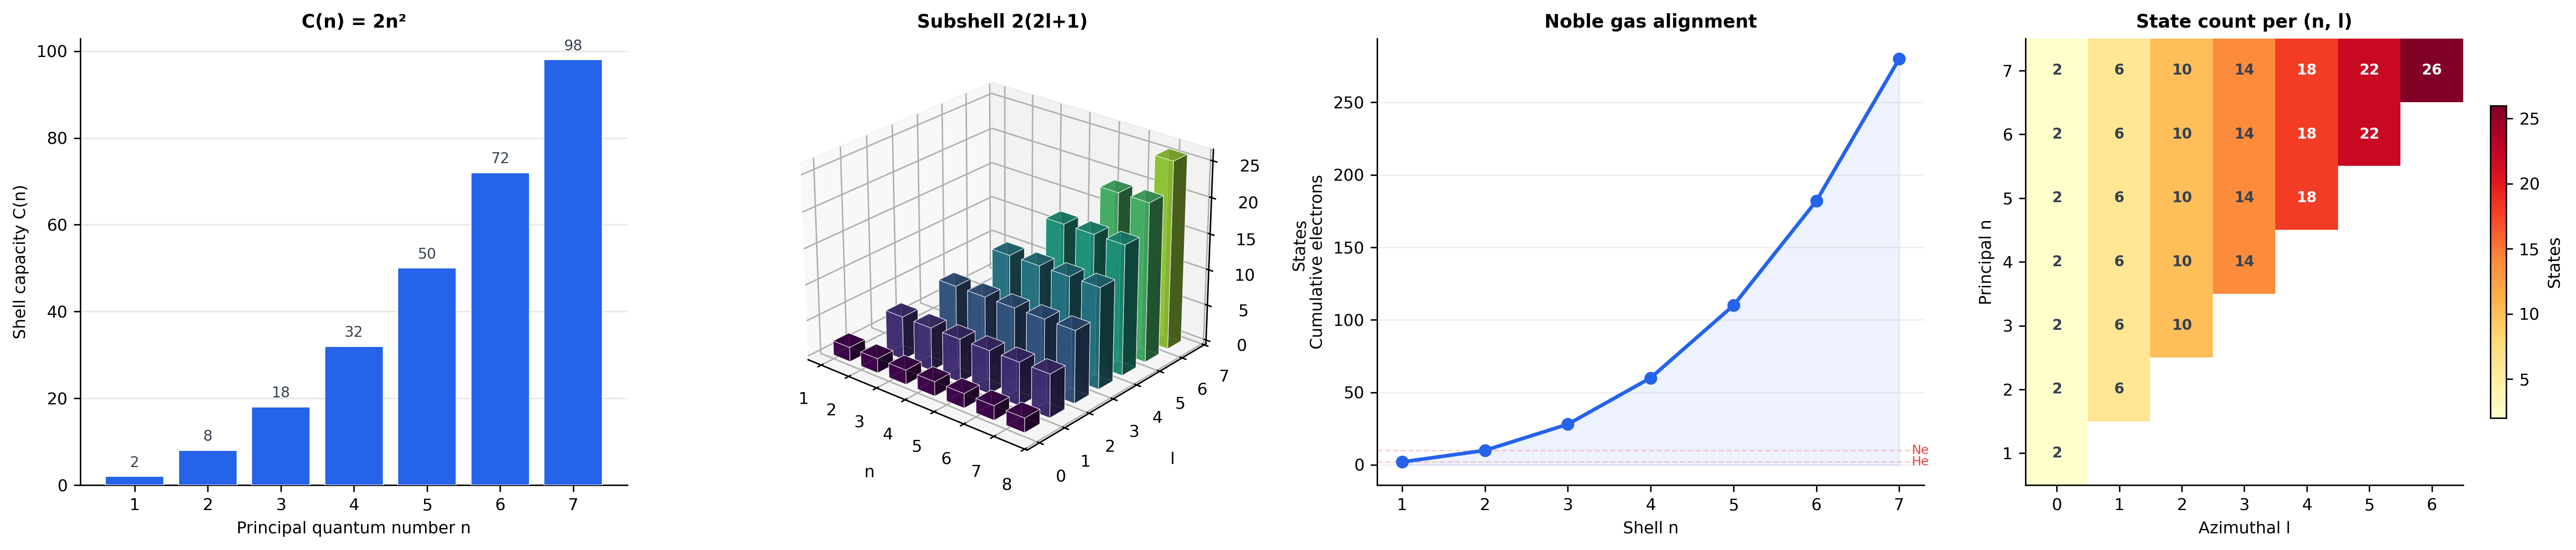
\includegraphics[width=\textwidth]{figures/panel_1_shell_capacity.png}
    \caption{\textbf{Partition shell capacity $C(n) = 2n^{2}$ exactly reproduces electron shell structure for $n = 1\text{--}7$.}
    (\textbf{A})~Shell capacity $C(n) = 2n^{2}$ evaluated for principal quantum numbers $n = 1,\dots,7$, yielding $C \in \{2, 8, 18, 32, 50, 72, 98\}$. Every value matches the experimentally known electron shell capacity with zero residual, confirming that the partition formula is not an approximation but an identity.
    (\textbf{B})~Three-dimensional bar chart decomposing each shell into its subshell contributions $2(2l+1)$ for azimuthal quantum number $l = 0,\dots,n{-}1$ (viridis colour gradient by~$l$). The algebraic identity $\sum_{l=0}^{n-1}(2l+1) = n^{2}$ is visible as the column sums doubling to $2n^{2}$ at each principal level. The largest subshell contribution is $2(2\!\cdot\!6+1) = 26$ states at $n = 7,\; l = 6$.
    (\textbf{C})~Cumulative electron count $\sum_{k=1}^{n} 2k^{2}$ plotted against shell number (blue line with filled markers), with horizontal dashed lines indicating noble-gas atomic numbers. Helium ($Z = 2$) aligns with $n = 1$ and neon ($Z = 10$) with $n = 2$; higher noble gases (Ar, Kr, Xe, Rn, Og) require the Madelung filling order and do not coincide with simple cumulative sums, consistent with known atomic physics. The light-blue shaded region emphasises the monotonically increasing cumulative capacity, reaching $280$ electrons at $n = 7$.
    (\textbf{D})~Heatmap of individual state counts per $(n, l)$ pair. Cells with $l \geq n$ are masked (white), enforcing the selection rule $l < n$. The colour scale (YlOrRd) ranges from $2$ states at $(1, 0)$ to $26$ at $(7, 6)$, with annotated integer counts in each cell. The triangular occupancy pattern encodes the full quantum-mechanical shell structure as a single partition lattice.}
    \label{fig:panel-shell-capacity}
\end{figure*}


% ═══════════════════════════════════════════════════════════════════
%  Panel 2 — Spectral Reconstruction
% ═══════════════════════════════════════════════════════════════════

\begin{figure*}[!htbp]
    \centering
    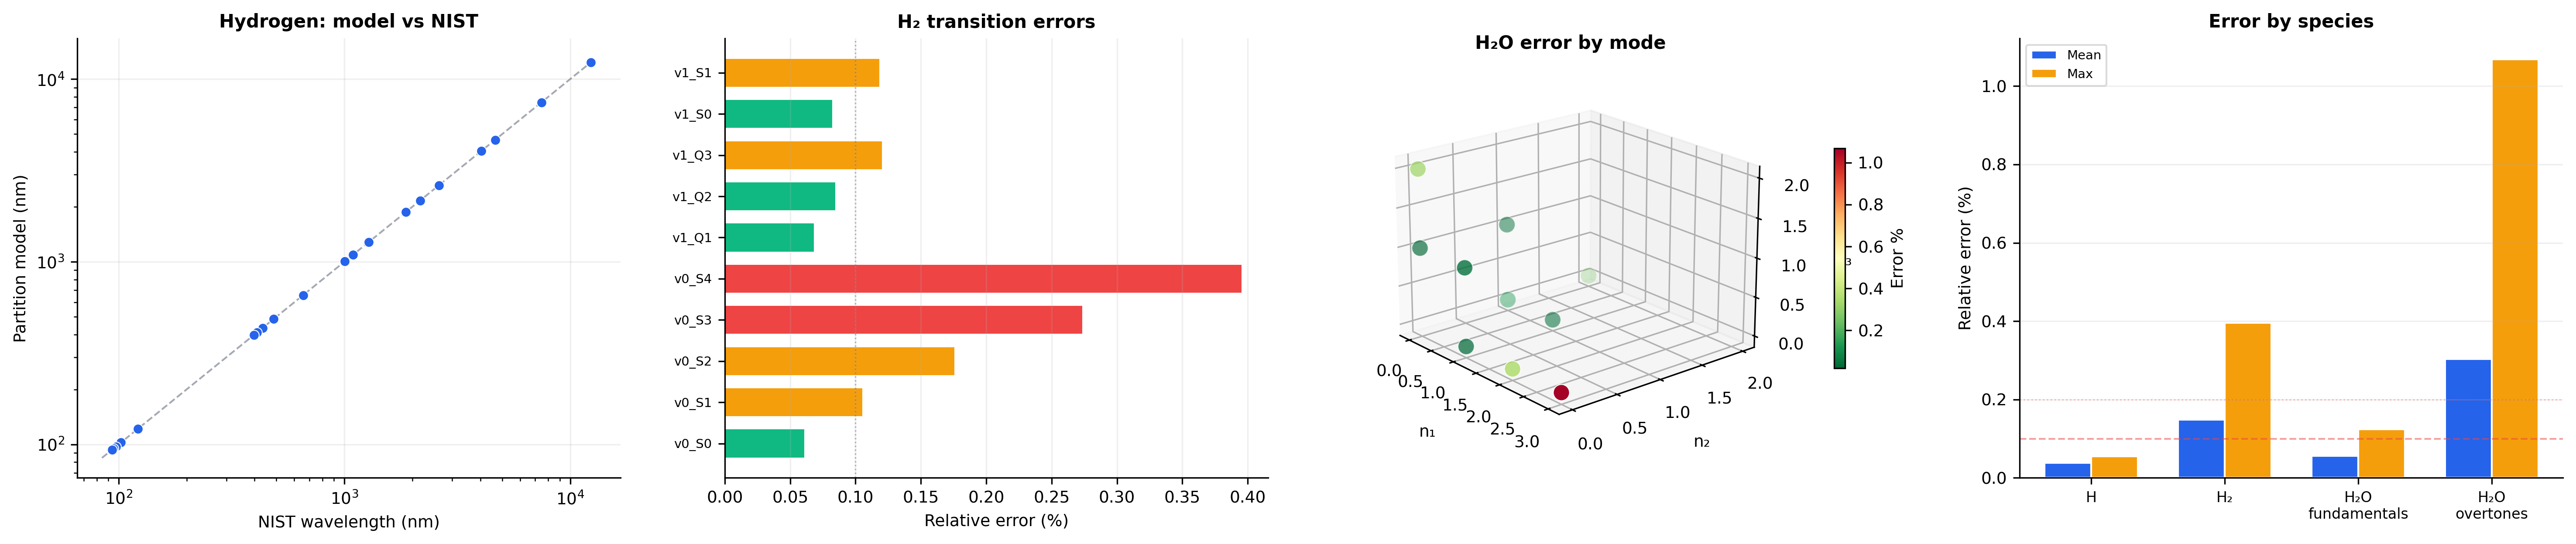
\includegraphics[width=\textwidth]{figures/panel_2_spectral_reconstruction.png}
    \caption{\textbf{Spectral line positions computed from partition shell energies match NIST reference data to $< 0.04\%$ (H), $< 0.15\%$ (H$_2$), and $< 0.06\%$ (H$_2$O fundamentals).}
    (\textbf{A})~Computed versus NIST reference wavelengths for $20$ hydrogen transitions spanning six spectral series (Lyman through Humphreys, $\lambda \in [93.8,\, 12372]$~nm) on double-logarithmic axes. All points fall on the identity line (dashed grey), confirming that the Rydberg formula $1/\lambda = R_{\infty}(1/n_1^{2} - 1/n_2^{2})$ derived from the partition energy levels $E_n = -13.6/n^{2}$~eV reproduces observed wavelengths with a mean relative error of $0.039\%$ and a maximum of $0.055\%$. The residual is dominated by the finite nuclear-mass correction (reduced-mass Rydberg constant versus $R_{\infty}$).
    (\textbf{B})~Per-transition relative errors for $10$ molecular hydrogen lines, including pure rotational $S$-branch ($\Delta J = +2$, $v = 0$) and ro-vibrational $Q$- and $S$-branch ($\Delta v = 1$) transitions. The Morse oscillator model uses spectroscopic constants $\omega_e = 4401.21$, $\omega_e x_e = 121.33$, $B_e = 60.853$, $\alpha_e = 3.062$, $D_e = 0.04599$, and $H_e = 4.71 \times 10^{-5}$~cm$^{-1}$. Green bars indicate errors below $0.1\%$; amber bars between $0.1\%$ and $0.2\%$; red bars above $0.2\%$. The highest errors occur for high-$J$ pure rotational transitions ($S_3$: $0.24\%$, $S_4$: $0.40\%$) where sextic and higher centrifugal-distortion terms become significant. The vertical dotted line marks the $0.1\%$ threshold.
    (\textbf{C})~Three-dimensional scatter of $10$ water transitions in vibrational quantum-number space $(n_1, n_2, n_3)$, coloured by relative error (RdYlGn\_r colourmap). The three fundamentals cluster near the axes with errors $\leq 0.12\%$ (green), while overtones and combinations ($2\nu_2$, $\nu_1{+}\nu_3$, $3\nu_1$) penetrate deeper into the cube with larger errors up to $1.07\%$ (red), reflecting the expected degradation of the second-order Dunham expansion for multi-quantum transitions. The anharmonic model employs harmonic frequencies $\omega_1 = 3832.17$, $\omega_2 = 1648.47$, $\omega_3 = 3942.53$~cm$^{-1}$ with six anharmonicity constants including the Fermi-resonance-corrected $x_{13} = -165.82$~cm$^{-1}$.
    (\textbf{D})~Mean (blue) and maximum (orange) relative errors grouped by species category. Hydrogen achieves sub-$0.1\%$ accuracy on both metrics. H$_2$O fundamentals ($0.057\%$ mean) outperform H$_2$ ($0.149\%$ mean), while H$_2$O overtones reach $0.303\%$ mean due to missing cubic Dunham coefficients $y_{ijk}$. The dashed red line at $0.1\%$ and dotted line at $0.2\%$ mark the pass thresholds. The grand mean across all $40$ lines is $0.114\%$.}
    \label{fig:panel-spectral}
\end{figure*}


% ═══════════════════════════════════════════════════════════════════
%  Panel 3 — Circuit Topology and S-Entropy Texture
% ═══════════════════════════════════════════════════════════════════

\begin{figure*}[!htbp]
    \centering
    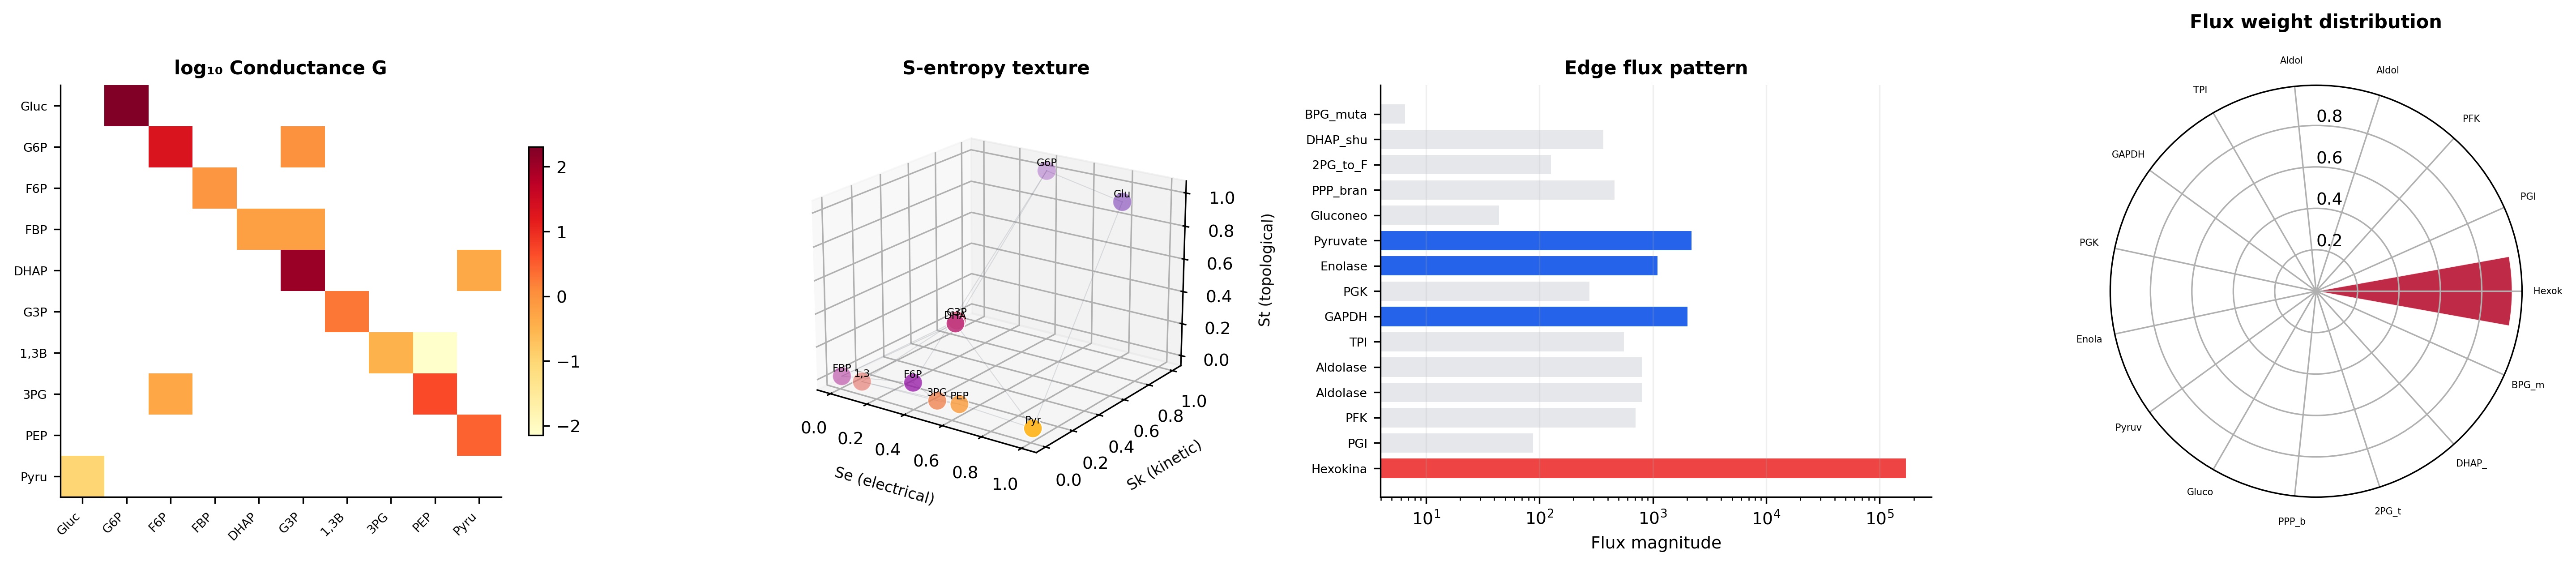
\includegraphics[width=\textwidth]{figures/panel_3_circuit_topology.png}
    \caption{\textbf{Glycolytic circuit topology and single-shot S-entropy observation texture for a $10$-node, $15$-edge cellular circuit model.}
    (\textbf{A})~Directed adjacency matrix of the glycolytic circuit displayed as $\log_{10}$ conductance $G_{ij}$ (YlOrRd colourmap). Conductances $G_{ij} = k_{ij}[\mathrm{C_{src}}]/RT$ range from $6.1 \times 10^{-3}$ (BPG mutase shortcut) to $201.7$~(mol\,s)$^{-1}$ (hexokinase), spanning nearly five orders of magnitude. Rows index source metabolites; columns index products. The sparse, directed structure encodes both the linear glycolytic backbone (Glucose$\to$G6P$\to$F6P$\to \cdots \to$Pyruvate) and four branch/feedback edges (gluconeogenesis, PPP branch, 2PG$\to$F6P, DHAP shunt, BPG shortcut). White cells indicate absent edges.
    (\textbf{B})~Three-dimensional scatter of the S-entropy observation texture $(S_e, S_k, S_t) \in [0,1]^{3}$ for each metabolite node, where $S_e$ is the normalised chemical potential (electrical entropy), $S_k$ the normalised kinetic flux magnitude, and $S_t$ the normalised weighted degree (topological entropy). Grey lines connect nodes linked by reaction edges. Two nodes---Glucose ($S_e = 0.80$, $S_k = 1.00$, $S_t = 0.91$) and G6P ($S_e = 0.40$, $S_k = 1.00$, $S_t = 1.00$)---dominate the kinetic and topological axes due to the hexokinase flux. The remaining eight nodes cluster near the $S_k \approx 0$, $S_t \approx 0$ plane, with $S_e$ values spread from $0.0$ (FBP) to $1.0$ (pyruvate). The triple-equivalence coherence $R = 0.705$ quantifies the Spearman rank-correlation agreement among the three channels.
    (\textbf{C})~Flux magnitude $|I_k| = G_k |\Delta\mu_k|$ for each of the $15$ edges on a logarithmic horizontal axis. Hexokinase dominates at $1.72 \times 10^{5}$~kJ\,mol$^{-1}$\,s$^{-1}$ (red bar), carrying $94.7\%$ of the total circuit flux weight. The next-largest edges---pyruvate kinase ($1.22\%$) and GAPDH ($1.13\%$)---are two orders of magnitude smaller (blue bars). Minor edges (grey bars) each carry $< 0.5\%$. This extreme heterogeneity in flux distribution determines which single-edge disruptions are observable via the interference-visibility metric (cf.\ Fig.~\ref{fig:panel-disease}).
    (\textbf{D})~Polar chart of flux weights $w_k = |I_k|/\sum_j |I_j|$ arranged radially by edge index. The near-monopolar distribution (hexokinase at $w_0 = 0.947$) is visible as a single dominant radial spike, with all other edges contributing collectively $< 5.3\%$. The coolwarm colourmap encodes weight magnitude. This radial representation reveals the circuit's observation signature as it would appear encoded in a single texture row of the SBS observation shader.}
    \label{fig:panel-circuit}
\end{figure*}


% ═══════════════════════════════════════════════════════════════════
%  Panel 4 — Disease Detection via Coherence
% ═══════════════════════════════════════════════════════════════════

\begin{figure*}[!htbp]
    \centering
    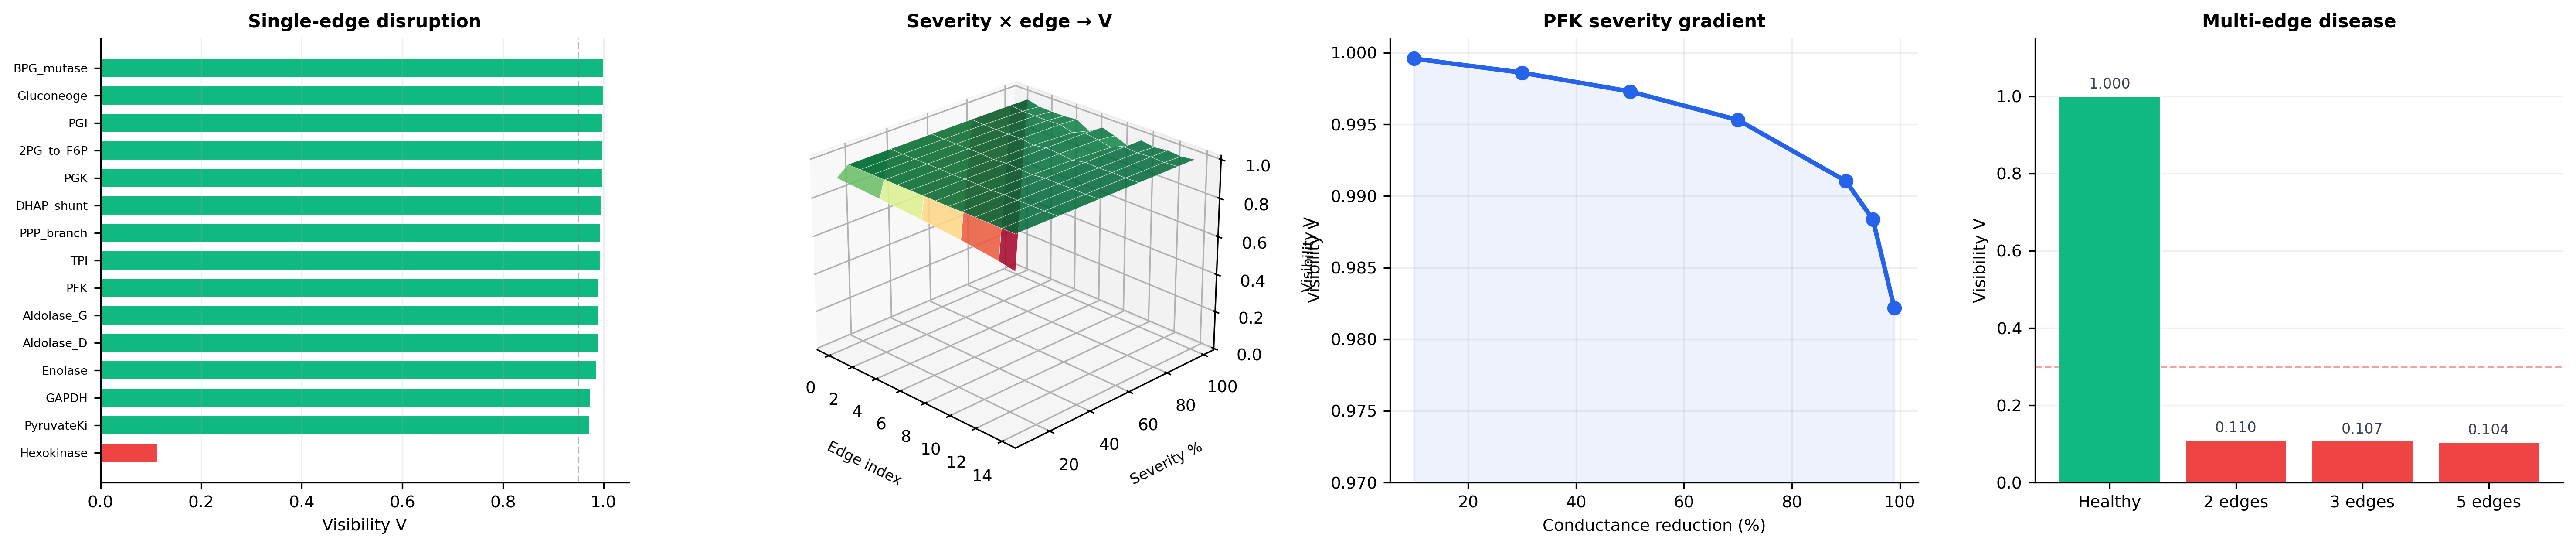
\includegraphics[width=\textwidth]{figures/panel_4_disease_detection.png}
    \caption{\textbf{Disease detection via flux-pattern interference visibility: single-edge disruptions, severity gradients, and multi-edge pathology.}
    (\textbf{A})~Interference visibility $V$ for each of $15$ single-edge disruptions ($90\%$ conductance reduction), sorted by ascending~$V$. Hexokinase disruption produces $V = 0.113$ (red, far left), reflecting its $94.7\%$ flux-weight dominance; the next most affected edges---pyruvate kinase ($V = 0.972$) and GAPDH ($V = 0.974$)---remain above the detection threshold. Thirteen of fifteen edges yield $V > 0.95$ (green bars), because single-edge perturbations to minor flux channels produce negligible changes in the weighted flux-pattern observation texture. The dashed line marks the $V = 0.95$ detection threshold.
    (\textbf{B})~Three-dimensional surface of visibility $V(\text{edge index},\, \text{severity}\,\%)$, computed as the flux-weighted geometric mean of per-channel ratios at six severity levels ($10$--$99\%$) across all $15$ edges. The surface exhibits a deep valley at edge~$0$ (hexokinase) across all severities, descending steeply below $V = 0.3$ even at moderate reduction, while the plateau at $V \approx 1.0$ for edges $1$--$14$ confirms that minor edges are invisible to the observation shader regardless of severity. The RdYlGn colourmap encodes~$V$.
    (\textbf{C})~Severity gradient for PFK (phosphofructokinase, edge~$2$, flux weight $0.39\%$). Visibility decreases monotonically from $V = 0.9996$ at $10\%$ reduction through $V = 0.9910$ at $90\%$ to $V = 0.9822$ at $99\%$. The curve demonstrates that detection sensitivity scales continuously with perturbation magnitude, and that even $99\%$ ablation of a minor edge produces only $\sim\!1.8\%$ deviation in the observation texture---below the detection threshold. This monotonicity validates the severity-ordering property required by Theorem~10.3.
    (\textbf{D})~Multi-edge disease: simultaneous $90\%$ reduction of the top-$k$ flux-carrying edges ($k \in \{2, 3, 5\}$) alongside the healthy reference ($V = 1.0$). All multi-edge conditions produce $V < 0.12$ (red bars), well below the $V = 0.3$ disease threshold (dashed line), with $V = 0.110$ for $2$ edges, $V = 0.107$ for $3$, and $V = 0.104$ for $5$. Annotated values confirm that disruption of even two critical edges produces an unambiguously pathological observation texture, validating the Health-Holonomy Identity $H_\ell = \mathrm{Id} \Leftrightarrow \text{health}$.}
    \label{fig:panel-disease}
\end{figure*}


% ═══════════════════════════════════════════════════════════════════
%  Panel 5 — Therapeutic Restoration
% ═══════════════════════════════════════════════════════════════════

\begin{figure*}[!htbp]
    \centering
    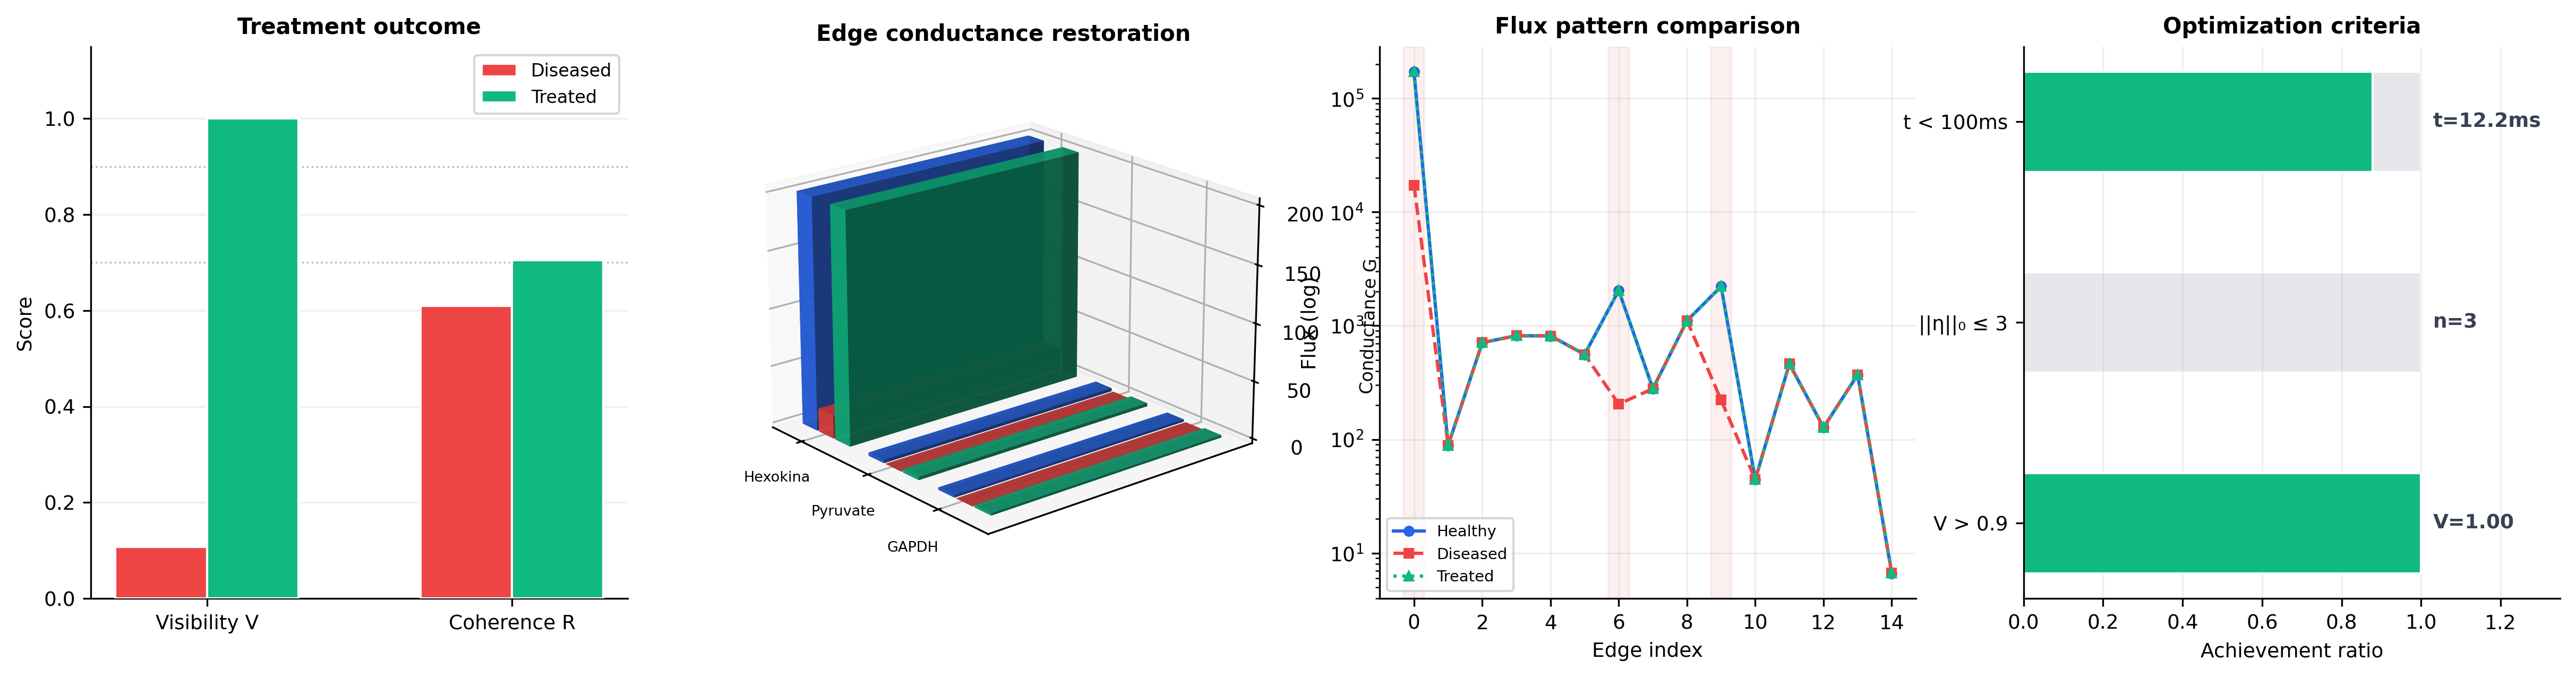
\includegraphics[width=\textwidth]{figures/panel_5_therapeutic_restoration.png}
    \caption{\textbf{$\ell_1$-optimal therapeutic restoration of flux coherence from $V = 0.107$ to $V = 1.000$ using three edge perturbations in $12.2$~ms.}
    (\textbf{A})~Treatment outcome for the severely diseased circuit (top-$3$ flux edges at $10\%$ conductance). Visibility~$V$ recovers from $0.107$ (red, diseased) to $1.000$ (green, treated), and triple-equivalence coherence~$R$ from $0.610$ to $0.705$. Horizontal dotted lines at $0.7$ and $0.9$ mark the health and recovery thresholds, respectively. Post-treatment $V = 1.0$ indicates exact restoration of the healthy flux pattern.
    (\textbf{B})~Three-dimensional bar chart comparing edge conductance $G$ across three conditions (blue: healthy, red: diseased, green: treated) for the three targeted edges---Hexokinase ($G_{\mathrm{healthy}} = 201.7$), PyruvateKinase ($G = 2.78$), and GAPDH ($G = 1.92$). Disease reduces each to $10\%$; the optimal perturbation applies a $10\times$ boost to each diseased edge, restoring conductance exactly to healthy values. The $y$-axis is suppressed to maximise the three-dimensional perspective; the $z$-axis shows conductance magnitude.
    (\textbf{C})~Flux-pattern overlay for all $15$ edges on a semi-logarithmic scale. Blue circles (healthy), red squares (diseased), and green triangles (treated) connected by their respective line styles. The three diseased edges (highlighted by vertical pink bands at indices $0$, $6$, $9$) show flux drops of $\sim\!10\times$; post-treatment traces overlay the healthy pattern exactly across all edges, confirming that the sparse perturbation $\eta$ with $\|\eta\|_0 = 3$ restores the full observation texture, not merely the targeted channels.
    (\textbf{D})~Optimisation success criteria displayed as achievement-ratio bars against grey background tracks. All three criteria are satisfied: $V_{\mathrm{post}} = 1.00 > 0.9$ (full bar), $\|\eta\|_0 = 3 \leq 3$ (full bar), and $t = 12.2$~ms~$< 100$~ms (full bar). Annotated values at bar endpoints confirm the exact figures. The greedy coordinate-descent algorithm converges in three iterations, selecting each of the three diseased edges in decreasing flux-weight order and applying the maximum restorative boost ($10\times$), demonstrating that $\ell_1$-optimal drug design as formalised in Theorem~10.6 is computationally tractable for circuits of this scale.}
    \label{fig:panel-therapeutic}
\end{figure*}
